%COPYRIGHT
%SHERMAN IP 2018

\documentclass[10pt]{proc}
%\usepackage[a4paper, total={15cm, 20cm}]{geometry}

\usepackage{amsmath}
\usepackage{amsthm}
\usepackage{amssymb}
\usepackage{amsbsy}
\usepackage{graphicx}
\usepackage{natbib}
\usepackage{url}
\usepackage{subcaption}
\usepackage[nottoc]{tocbibind}
\usepackage[bookmarks=true]{hyperref}
\usepackage{bookmark}
\usepackage{hyphenat}
\usepackage{listings}
\lstset{basicstyle=\ttfamily,breaklines=true}
%\usepackage{rotating}
\usepackage{color} %red, green, blue, yellow, cyan, magenta, black, white
\usepackage[dvipsnames]{xcolor}
\usepackage{epstopdf}

\definecolor{mygreen}{RGB}{28,172,0} % color values Red, Green, Blue
\definecolor{mylilas}{RGB}{170,55,241}
\definecolor{bck}{RGB}{239,240,241}

\DeclareMathOperator{\expfamily}{ExpFamily}
\DeclareMathOperator{\expectation}{\mathbb{E}}
\DeclareMathOperator{\variance}{\mathbb{V}ar}
\DeclareMathOperator{\cov}{\mathbb{C}ov}
\DeclareMathOperator{\corr}{\mathbb{C}orr}
\DeclareMathOperator{\bernoulli}{Bernoulli}
\DeclareMathOperator{\betaDist}{Beta}
\DeclareMathOperator{\dirichlet}{Dir}
\DeclareMathOperator{\bin}{Bin}
\DeclareMathOperator{\MN}{Multinomial}
\DeclareMathOperator{\prob}{\mathbb{P}}
\DeclareMathOperator{\trace}{Tr}
\DeclareMathOperator{\normal}{N}
\DeclareMathOperator{\gammaDist}{Gamma}
\DeclareMathOperator{\poisson}{Poisson}

\newcommand{\RSS}{\mathrm{RSS}}
\newcommand{\euler}{\mathrm{e}}
\newcommand{\diff}{\mathrm{d}}
\newcommand{\T}{^\textup{T}}
%\newcommand{\dotdotdot}{_{\phantom{.}\cdots}}
\newcommand{\dotdotdot}{...}
\newcommand{\BIC}{\textup{BIC}}

\newcommand{\vect}[1]{\mathbf{#1}}
\newcommand{\vectGreek}[1]{\boldsymbol{#1}}
\newcommand{\matr}[1]{\mathsf{#1}}

\newtheorem{theorem}{Theorem}
\newtheorem{algorithm}{Algorithm}

\author{Sherman Ip - September 2018}
\title{A Review of Fusion Energy, Metropolis Hastings, Hamiltonian Monte Carlo and the No U-Turn Sampler}

\begin{document}\sloppy

\maketitle

\section{Fusion Energy}
A review of nuclear fusion will be given here. Most of the fundamental maths and physics here are covered in undergraduate textbooks such as \cite{riley2006mathematical}, \cite{serway2018physics} and \cite{martin2006nuclear}. Advanced topics in tomamkas are covered in \cite{wesson2004tokamaks}.

An example of nuclear fusion is the fusion of deuterium $_{2}^{1}\textrm{H}$ and tritium $_{3}^{1}\textrm{H}$ atoms in the following reaction
\begin{equation}
  ^{2}_{1}\textrm{H} + ^{3}_{1}\textrm{H} \rightarrow
  ^{1}_{0}\textrm{n} + ^{4}_{2}\textrm{He} \ .
\end{equation}
High temperatures of $\sim 10^8 \text{K}$ are required for the fusion reaction to occur by overcoming the Coulomb barrier. In this reaction, the kinetic energy of the $\alpha$ particle and the neutron are 3.5 MeV and 14.1 MeV respectively. The energy can be harnessed using neutron absorbing material such as lithium.

At such high temperatures, atoms are ionized to form plasma. and this must be contained for the purpose of fusion energy. A tokamak, a doughnut-like shaped container, contains the plasma using magnetic coils which forms a helical magnetic field.

Achieving ignition, that is when the power generated is greater than the rate of energy lost, is difficult to achieve. The Lawson's criterion \citep{lawson1957some} describes that high ion density and high confinement time are required for ignition.

The plasma with charge density vector field $\mathbf{j}$ interacts with the magnetic vector field $\mathbf{B}$. For high confinement time, the force exerted by the magnetic field must balance with the outward pressure scalar field, $p$, of the plasma; this is known as the equilibrium state. A description of the equilibrium state can be obtained from Maxwell's equations
\begin{equation}
  \mu_0\mathbf{j}=\nabla \times \mathbf{B}
\end{equation}
\begin{equation}
  \nabla \cdot \mathbf{B} = 0
\end{equation}
and the force density
\begin{equation}
  \mathbf{j}\times\mathbf{B} = \nabla p \ .
\end{equation}

Axis symmetry was assumed here so that a poloidal cross section of the tokamak is only relevant. A further definition can be made to simplify future calculations. Using the magnetic potential $\mathbf{A}$, then
\begin{equation}
  \mathbf{B} = \nabla \times \mathbf{A}
\end{equation}
which in cylindrical coordinates $(r,\phi,z)$ is
\begin{equation}
  \mathbf{B} = 
  \dfrac{1}{r}
  \left \|\begin{matrix}
  \widehat{\mathbf{e}}_r & \partial/\partial r & A_r \\
  r \widehat{\mathbf{e}}_\phi & \partial/\partial\phi & rA_\phi \\
  \widehat{\mathbf{e}}_z & \partial/\partial z & A_z
  \end{matrix}\right \| \ .
\end{equation}
Because of axis symmetry, the poloidal magnetic field is
\begin{equation}
  \mathbf{B_p} = -\dfrac{1}{r}\dfrac{\partial \psi}{\partial z}\widehat{\mathbf{e}}_r + \frac{1}{r}\dfrac{\partial\psi}{\partial r}\widehat{\mathbf{e}}_z
\end{equation}
where
\begin{equation}
\psi = rA_\phi
\end{equation}
is the poloidal magnetic flux function. Similarly the poloidal charge density is
\begin{equation}
  \mathbf{j_p} = -\dfrac{1}{r}\dfrac{\partial f}{\partial z}\widehat{\mathbf{e}}_r + \frac{1}{r}\dfrac{\partial f}{\partial r}\widehat{\mathbf{e}}_z
\end{equation}
where
\begin{equation}
  f = r B_\phi /\mu_0
\end{equation}
is the current flux function. It can be verified that these satisfy Maxwell's equations. The poloidal magnetic and charge density can be rewritten as
\begin{equation}
  \mathbf{B_p} = \dfrac{1}{r}\left(\nabla\psi\times\widehat{\mathbf{e}}_\phi\right)
  \label{eq:poloidal_magnetic}
\end{equation}
and
\begin{equation}
  \mathbf{j_p} = \dfrac{1}{r}\left(\nabla f\times\widehat{\mathbf{e}}_\phi\right)
  \label{eq:poloidal_current}
\end{equation}
respectively.

Again in cylindrical coordinates, assuming axis symmetry and $(\nabla p)\cdot\widehat{\mathbf{e}}_\phi=0$, the force density is
\begin{equation}
  \mathbf{j}\times\mathbf{B} =
  B_\phi\left(\mathbf{j_p}\times\widehat{\mathbf{e}}_\phi\right)
  +j_\phi\left(\widehat{\mathbf{e}}_\phi\times\mathbf{B_p}\right) \ .
\end{equation}
Using Equations \eqref{eq:poloidal_magnetic} and \eqref{eq:poloidal_current}, with the triple vector product $\mathbf{a}\times(\mathbf{b}\times\mathbf{c}) = (\mathbf{c}\cdot\mathbf{a})\mathbf{b} - (\mathbf{a}\cdot\mathbf{b})\mathbf{c}$, then
\begin{equation}
  \nabla p = -\dfrac{f\mu_0}{r^2}\nabla f+\dfrac{j_\phi}{r}\nabla \psi \ .
\end{equation}
Using the chain rule
\begin{equation}
\dfrac{\diff p}{\diff \psi} = \dfrac{\partial p}{\partial z}\dfrac{\diff z}{\diff \psi} + \dfrac{\partial p}{\partial r}\dfrac{\diff r}{\diff \psi}
\end{equation}
then
\begin{equation}
j_\phi = r\dfrac{\diff p}{\diff \psi}+\dfrac{\mu_0}{r}f\dfrac{\diff f}{\diff \psi} \ .
\label{eq:j_psi}
\end{equation}

Using the fact that $\mu_0j_\phi=\left(\nabla\times\mathbf{B}\right)\cdot\widehat{\mathbf{e}}_\phi$ then
\begin{equation}
  \mu_0j_\phi = -\dfrac{1}{r}\dfrac{\partial^2\psi}{\partial z^2}-\dfrac{\partial}{\partial r}
    \left(
      \dfrac{1}{r}\dfrac{\partial\psi}{\partial r}
    \right)
  \ .
\end{equation}
This can be combined with Equation \eqref{eq:j_psi} to get the Grad-Shafranov equation \citep{grad1958hydromagnetic} \citep{shafranov1966plasma}
\begin{equation}
\dfrac{\partial^2 \psi}{\partial z^2}+r\dfrac{\partial}{\partial r}\left(\dfrac{1}{r}\dfrac{\partial\psi}{\partial r}\right)
=
-r^2\mu_0\dfrac{\diff p}{\diff \psi}-\mu_0^2f\dfrac{\diff f}{\diff \psi}
\ .
\end{equation}
The Grad-Shafranov equation can be solved numerically, for example to solve for the current density spatially in a tokamak \citep{lao1985reconstruction}. This is known as the equilibrium problem.

Current tomography divides the tokamak cross section into a grid and solves for each grid element the current density under the equilibrium problem given measurements or diagnostics \citep{svensson2008current}. Diagnostics include the magnetic field strength from and of the coils, temperature readings and particles undergoing Thomson scattering \citep{svensson2004integrating} \citep{ford2009bayesian}. This can quickly turn into a high dimensional problem. By connecting all of the diagnostics and ingredients of the Grad-Shafranov equation together, a hierarchical model can be built. Bayesian inference can be used on the hierarchical model to make predictions, along with error bars, variables of interest such as the current density. There exist software which builds such a hierarchical model \citep{svensson2007large} \citep{svensson2008current} \citep{svensson2010connecting}. However exact methods for Bayesian inference is  very hard and approximate methods such as MCMC are required here \citep{ford2010tokamak}.

\section{Metropolis Hastings}
Bayesian inference is the study of the posterior distribution, for example the posterior distribution can be $\mathbf{X} = j_\phi\text{ for all grid elements}|\text{diagnostics}$. The aim of Markov chains using Monte Carlo (MCMC) is to simulate the posterior distribution, otherwise known as sampling the target distribution. Suppose the MCMC samples are $\mathbf{X}_0,\mathbf{X}_1,\dotdotdot\mathbf{X}_n$, then useful summary statistics can be obtained such as the mean
\begin{equation}
\widehat{\vectGreek{\mu}} = \dfrac{1}{n}\sum_{i=1}^n \mathbf{X}_i
\end{equation}
and the covariance
\begin{equation}
\widehat{\matr{\Sigma}} = \dfrac{1}{n-1}\sum_{i=1}^n \left[\mathbf{X}_i-\widehat{\vectGreek{\mu}}\right]
\left[\mathbf{X}_i-\widehat{\vectGreek{\mu}}\right]\T
\end{equation}
which can be used to obtain error bars. To make sampling easier, MCMC sample samples which are Markovian $\{\mathbf{X}_n|\mathbf{X}_{n-1},\mathbf{X}_{n-2},\dotdotdot,\mathbf{X}_{0}\} = \{\mathbf{X}_n|\mathbf{X}_{n-1}\}$.

The random walk Metropolis-Hastings (RWMH) algorithm \citep{metropolis1953equation} \citep{hastings1970monte} is an example of a MCMC. Suppose a sample $\vect{X}_n = \vect{x}_n$ was obtained. Define the proposal to be $\vect{Y}_{n+1}|\vect{X}_n=\vect{x}_n \sim \normal\left(\vect{x}_n,\matr{\Theta}\right)$ which is a random walk. The transition from $\vect{X}_n=\vect{x}_n$ to $\vect{X}_{n+1}$ is
\begin{multline}
\vect{X}_{n+1}|\vect{Y}_{n+1} = \vect{y}_{n+1}, \vect{X}_{n} = \vect{x}_n
\\= 
	\begin{cases}
	\vect{y}_{n+1} & \text{with probability } \alpha\left(\vect{x}_n,\vect{y}_{n+1}\right) \\
	\vect{x}_n & \text{otherwise}
	\end{cases}
\end{multline}
where
\begin{equation}
\alpha\left(\vect{x}_{n},\vect{y}_{n+1}\right)=\min\left(1,\dfrac{\pi(\vect{y}_{n+1})}{\pi(\vect{x}_{n})}\right)
\end{equation}
is the acceptance rate and $\pi(\vect{x})$ is the target density function. Suppose $\vect{X}_0=\vect{x}_0$ was defined or selected by the user, then the samples $\vect{X}_1,\vect{X}_2,\dotdotdot$ can be obtained. It can be shown that under mild conditions, such a transition will make the Markov chain converge to, or sample correctly, the target distribution \citep{roberts1994simple}.

The proposal covariance $\matr{\Theta}$ must be selected however and this does affect the acceptance rate and the performance of the RWMH. Acceptance rates too small or too large will cause the chain to not explore the target well \citep{gelman1996efficient}. Under some strong assumptions and in high dimension $d$, the optimal acceptance rate is about 0.234 \citep{gelman1996efficient} \citep{roberts1997weak} \citep{rosenthal2011optimal}. In the Gaussian example, the optimial covariance is $\matr{\Theta}={2.38^2}\matr{\Sigma}/d$ where $\matr{\Sigma}$ is the covariance of the target.

$\matr{\Sigma}$ is usually unknown. There exist adaptive methods \citep{haario2001adaptive} \citep{roberts2009examples} which adapts $\matr{\Theta}$ on the go. Let the proposal be $\vect{Y}_{n+1}|\vect{X}_n=\vect{x}_n\sim \normal\left(\vect{x}_n,\matr{\Theta}_n\right)$. The adaptive RWMH sets $\matr{\Theta}_{n}=\matr{\Theta}_0$ for $n<n_0$, otherwise
\begin{equation}
\matr{\Theta}_{n} =
\begin{cases}
2.38^2 \widehat{\matr{\Sigma}}_n/d & \text{with probability }1-\beta \\
\matr{\Theta}_0 & \text{otherwise}
\end{cases}
\end{equation}
where $\matr{\Theta}_0$ is some small initial proposal covariance, $n_0$ is an integer determining the number of initial non-adaptive steps, $\widehat{\matr{\Sigma}}_n$ is the unbiased sample covariance estimator of the chain $\vect{X}_0,\vect{X}_1,\dotdotdot,\vect{X}_n$ and $0\leqslant\beta\leqslant 1$ is some small number \citep{roberts2009examples}. For example it was selected that $n_0= 2d-1$ and $\beta = 0.05$. It can be shown that under some conditions, these adaptive methods will still sample the target correctly \citep{rosenthal2007coupling}.

\section{Hamiltonian Monte Carlo}
Hamiltonian Monte Carlo (HMC) \citep{neal2011mcmc} improves the random walk behaviour in RWMH by using Hamiltonian dynamics to guide the direction of the chain. The Hamilton's equations are
\begin{equation}
\dfrac{\diff x_i}{\diff t}=\dfrac{\partial H}{\partial p_i}
\qquad\&\qquad
\dfrac{\diff p_i}{\diff t}=\dfrac{\partial H}{\partial x_i}
\end{equation}
where $x_i$ and $p_i$ are components of the position and momentum vector respectively and $H$ is the Hamiltonian. Let $\matr{M}$ be a mass matrix which is symmetric and positive definite, then the Hamiltonian is
\begin{equation}
H(\vect{x},\vect{p})=U(\vect{x}) + \dfrac{1}{2}\vect{p}\T\matr{M}^{-1}\vect{p}
\end{equation}
where $U(\vect{x})$ is the potential energy. The potential energy for a target is given as
\begin{equation}
U(\vect{x}) = -\ln\pi(\vect{x})
\end{equation}
which comes from the Boltzmann's factor.

The algorithm requires the following parameters, a positive integer for number of leap frog steps $L$ and a positive number for the step size $\Delta t$. Suppose the chain is at $\vect{X}_n=\vect{x}_n$. Let $\vect{x}_n(0) = \vect{x}_n$. First a random momentum $\vect{p}_n(0)$ is drawn from $\normal\left(\vect{0},\matr{M}\right)$. Next the particle will run under Hamiltonian dynamics for time $L\Delta t$, this is done by solving the Hamilton's equations numerically using the leap frog algorithm. The equations required for the leap frog algorithm are:
\begin{equation}
\vect{p}_n\left(t+\dfrac{\Delta t}{2}\right) = \vect{p}_n(t) - \dfrac{\Delta t}{2}\nabla \left.U(\vect{x})\right|_{\vect{x} = \vect{x}_n(t)}
\label{eq:leapfrog1}
\end{equation}
\begin{equation}
\vect{x}_n(t+\Delta t) = \vect{x}_n(t)+\Delta t \matr{M}^{-1}\vect{p}_n\left(t+\dfrac{\Delta t}{2}\right)
\label{eq:leapfrog2}
\end{equation}
\begin{multline}
\vect{p}_n(t+\Delta t) =
\vect{p}_n\left(t+\dfrac{\Delta t}{2}\right)
\\
- \dfrac{\Delta t}{2}\nabla \left.U(\vect{x})\right|_{\vect{x} = \vect{x}_n(t+\Delta t)}
\ .
\label{eq:leapfrog3}
\end{multline}
Equations \eqref{eq:leapfrog1}, \eqref{eq:leapfrog2} and \eqref{eq:leapfrog3} are to be applied to $\vect{x}_n(0)$ and $\vect{p}_n(0)$ $L$ times to obtain $\vect{x}_n(L\Delta t)$ and $\vect{p}_n(L\Delta t)$.

Because the leap frog algorithm is a numerical method and does not solve the Hamilton's equations exactly, a Metropolis-Hastings step is used. The transition from $\vect{X}_n = \vect{x}_n$ to $\vect{X}_{n+1}$ is
\begin{multline}
\vect{X}_{n+1}|\vect{X}_{n}=\vect{x}_n
\\= 
	\begin{cases}
	\vect{x}_{n}(L\Delta t) & \text{with prob. } \alpha\left(\vect{x}_{n}(0),\vect{x}_{n}(L\Delta t)\right) \\
	\vect{x}_n(0) & \text{otherwise}
	\end{cases}
\end{multline}
where
\begin{multline}
\alpha\left(\vect{x}_{n}(0)_n,\vect{x}_{n}(L\Delta t)\right)=
\\
\min\left(
1,
\dfrac{
  \exp\left[
    -H(
      \vect{x}_n(L\Delta t),\vect{p}_n(L\Delta t)
    )
  \right]
}
{
  \exp\left[
    -H(
      \vect{x}_n(0),\vect{p}_n(0)
    )
  \right]
}
\right) \ .
\end{multline}

Because HMC improves on the random walk behaviour, HMC produce samples which are less correlated and explore the target well. There are a few disadvantages however, for example the parameters $\matr{M}$, $\Delta t$ and $L$ must be sensible for HMC to even work. There are strategies on tuning these parameters \citep{neal2011mcmc}. HMC also requires the derivative of the potential $\nabla U(\vect{x})$ which may not be available in closed form. Numerical differentiation is possible however HMC requires the partial derivative of every dimension at every leap frog, which can get computationally costly. Inaccuracies due to the numerical differentiation should automatically be taken care of in the Metropolis-Hastings step.

\section{No U-Turn Sampler}

The No U-Turn Sampler (NUTS) \citep{hoffman2014no} controls $L$ automatically. Tuning $L$ is critical. For example in the one dimensional $\normal(0,1/\sqrt{k})$ case the potential is $U(x)=kx^2/2$ which corresponds to the potential of a simple harmonic oscillator. For $L$ too large, the particle will oscillate and this waste computational time. For $L$ too small, the particle will behave like a random walk.

Loosely, NUTS runs the Hamiltonian dynamics both forwards and backwards in time randomly until a U-Turn condition is satisfied. When that happens, a random point from the path is chosen for the MCMC sample and the process is repeated from that new point.

In detail, a binary tree is constructed to trace the path of the leap frog steps. To produce a MCMC sample, an iterative procedure is conducted. A slice variable $U_n\sim\text{Uniform}(0,\exp(-H(\vect{x}_n(0),\vect{p}_n(0)))$ is sampled. Let $\vect{x}_n^+$ and $\vect{p}_n^+$ be the position and momentum of the forward particle respectively. Similarly $\vect{x}_n^-$ and $\vect{p}_n^-$ for the backward particle. In each iteration, the binary tree selects at random uniformly to move the forward particle forwards in time or the backward particle backwards in time. Also for each iteration, the number of leap frog steps increase by a factor of 2. For example in the first iteration the forward particle moves forwards in time using 1 leap frog step. In the next iteration the backward particle moves backwards in time using 2 leap frog steps.

The iterative procedure continues until the U-Turn condition is met, that is
\begin{equation}
(\vect{x}_n^+ - \vect{x}_n^-)\cdot \vect{p}_n^- < 0
\quad \text{or} \quad
(\vect{x}_n^+ - \vect{x}_n^-)\cdot \vect{p}_n^+ < 0
\end{equation}
or when the Hamiltonian becomes inaccurate
\begin{equation}
\exp\left[-H(\vect{x}_n^{+},\vect{p}_n^{+})+\delta\right]<U_n
\end{equation}
or
\begin{equation}
\exp\left[-H(\vect{x}_n^{-},\vect{p}_n^{-})+\delta\right]<U_n
\end{equation}
where for example $\delta = 1000$.

Once the U-Turn condition is met, the next MCMC sample, $\vect{x}_{n+1}$, is obtained by sampling uniformly the leap frog path traced out by the binary tree $\{\vect{x}_n^-,\dotdotdot,\vect{x}_n(-\Delta t),\vect{x}_n(0),\vect{x}_n(\Delta t),\dotdotdot,\vect{x}_n^+\}$ which satisfies
\begin{equation}
U_n<\exp\left[-H(\vect{x_{n+1}},\vect{p_{n+1})}\right] \ .
\label{eq:slice}
\end{equation}
This is usually satisfied if the remaining HMC parameters are sensible.

\section{Diagnostics}
A small example will be given here. A MCMC has been constructed to estimate the current density of a cross section of a tokamak, modelled by a $3\times 3$ grid. A grid element will be studied here. This particular model has 205 dimensions. Diagnostics are presented here to judge the performance of the adaptive RWMH with initial covariance $10^{-6}/205 \times \matr{I}$ where $\matr{I}$ is the identity matrix. The chain initial point is at the maximum of the posterior and ran for 10\,000 iterations.

A slight adjustment was made to the adaptive RWMH in this example. A biased sample covariance was used rather than the unbiased version. It is given as
\begin{equation}
\widehat{\matr{\Sigma}}_n=\dfrac{\sum_{i=1}^n\left[\vect{x}_i-\widehat{\vectGreek{\mu}}_n\right]\left[\vect{x}_i-\widehat{\vectGreek{\mu}}_n\right]\T}{n}
\end{equation}
where
\begin{equation}
\widehat{\vectGreek{\mu}}_n = \dfrac{1}{n+1}\sum_{i=1}^n \vect{x}_i \ .
\end{equation}
This helps the covariance to be non-singular if not enough acceptance steps were taken due to a poor choice of the initial covariance.

A trace plot is a plot of the MCMC sample $x_1,x_2,\dotdotdot,x_n$ and it gives some indication on how the MCMC explore the state space, ideally exploring the space rapidly at each iteration with a sensible acceptance rate \citep{rosenthal2011optimal}. The acceptance rate should be monitored and values such as 0.234 in \cite{roberts1997weak} is a good rule of thumb. An example of a good trace plot is shown in Figure \ref{fig:trace}. The acceptance rate, shown in Figure \ref{fig:accept}, does converge but to a value other than 0.234. This may be fine as the result in \cite{roberts1997weak} does depend on strong assumptions, such as independence between dimensions.

\begin{figure}[ht]
  \centering
  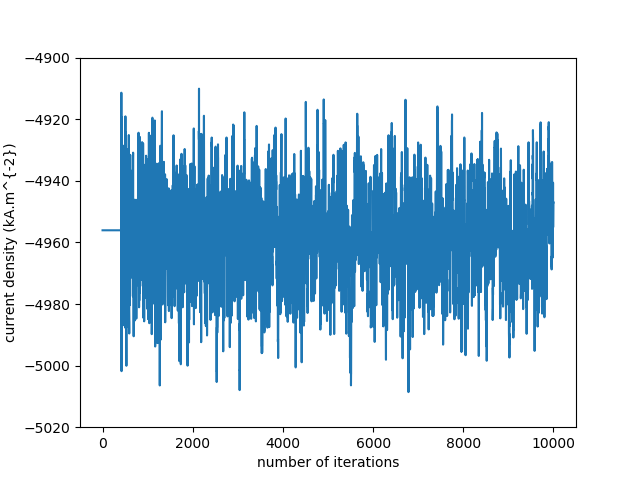
\includegraphics[width=0.45\textwidth]{chain_1.png}
  \caption{Trace plot of chain 1}
  \label{fig:trace}
\end{figure}
\begin{figure}[ht]
  \centering
  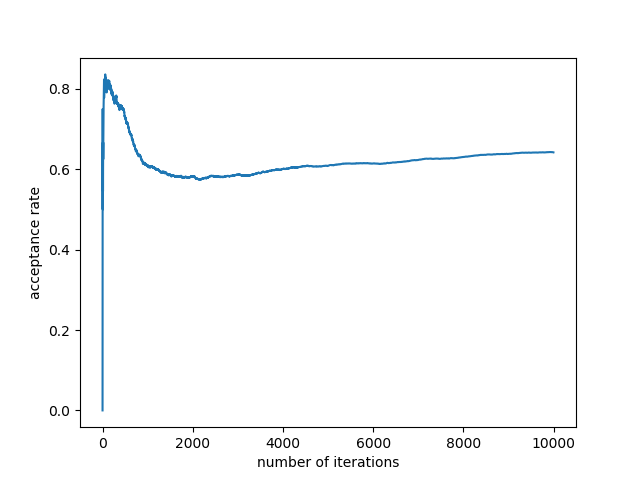
\includegraphics[width=0.45\textwidth]{accept.png}
  \caption{Acceptance rate of chain 1}
  \label{fig:accept}
\end{figure}

The autocorrelation \citep{geyer2011mcmc} indicates the correlation between MCMC samples. The autocorrelation with lag $k$ is
\begin{equation}
\widehat{\rho}(k)=\dfrac
{
  \sum_{i=1}^{n-k}(x_i-\bar{x})(x_{i+k}-\bar{x})
}
{
  \sum_{i=1}^{n}(x_i-\bar{x})^2
}
\end{equation}
where $\bar{x}=\sum_{i=1}^nx_i/n$. The autocorrelation should be as small as possible in magnitude as this would mean future samples won't be influenced as much by previous samples which may indicate how the MCMC explore the state space. If the samples are uncorrelated, then the autocorrelation should be $\|\widehat{\rho}(k)\|<1/\sqrt{n}$ for the majority of $k=1,2,3,\dotdotdot$. The autocorrelation is shown in Figure \ref{fig:acf} with low autocorrelation at around lag 40 and above.

\begin{figure}[ht]
  \centering
  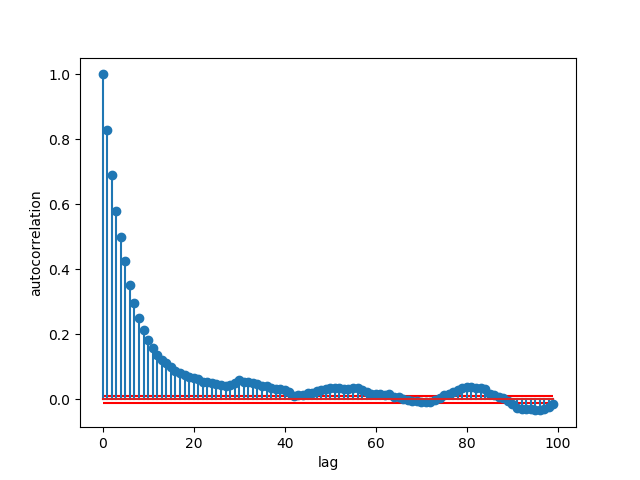
\includegraphics[width=0.45\textwidth]{acf.png}
  \caption{Autocorrelation of chain 1; red line = $\|{1/\sqrt{n}}\|$}
  \label{fig:acf}
\end{figure}

It may be convenient to combine the autocorrelation for different lags into a single number, the efficiency does that and is given as
\begin{equation}
\widehat{\text{efficiency}}=\left[1+2\sum_{i=1}^K\widehat{\rho}(i)\right]^{-1}
\end{equation}
where $K$ is the first odd positive integer for which $\widehat{\rho}(K + 1) + \widehat{\rho}(K + 2)$ is negative \citep{gelman2014bayesian}.

Burn-in \citep{geyer1992practical} \citep{geyer2011mcmc} is the discarding of samples at the start of the chain. This practice is done because the chain does need a number of iterations to converge to the target from some initial value and also for the adaptation to settle down. The Gelman-Rubin $F$ statistic \citep{gelman1992inference} is a rule of thumb for how many samples to discard for burn-in. This is done by starting multiple chains at different initial points and judging how long it takes for all of these chains to have similar sample means. The $F$ statistic is obtained by comparing the within and between chain variances using the second half of the chain, similar to the one-way ANOVA. Let $x_1^{(j)}, x_2^{(j)},\dotdotdot,x_n^{(j)}$ be the $j$th chain for $j=1,2,\dotdotdot,k$. Let
\begin{equation}
\bar{x}^{(j)}(n_b)=\dfrac{\sum_{i=n_b+1}^{2n_b}x_i^{(j)}}{n_b}
\end{equation}
and
\begin{equation}
\bar{x}^*(n_b) = \dfrac{\sum_{j=1}^k\sum_{i=n_b+1}^{2n_b}x_i^{(j)}}{kn_b}
\ .
\end{equation}
The within chain variance is
\begin{equation}
s_W^2(n_b) = \dfrac{
  \sum_{j=1}^k \sum_{i=n_b+1}^{2n_b} \left(
    x_i^{(j)} - \bar{x}^{(j)}(n_b)
  \right)^2
}
{
  kn - k
}
\end{equation}
and the between chain variance is
\begin{equation}
s_B^2(n_b) = \dfrac{
  \sum_{j=1}^k  n_b \left(
    \bar{x}^{(j)}(n_b) - \bar{x}^*(n_b)
  \right)^2
}
{
  k-1
}
\ .
\end{equation}
The $F$ statistic is
\begin{equation}
F(n_b) = s_B^2(n_b) / s_W^2(n_b) \ .
\end{equation}
The value of $n_b$ which makes $F$ closest to 1 is the amount of samples to discard for burn in. Unlike ANOVA though, the $F$ distribution cannot be used as independence cannot be assumed within chains. This implies that the $F$ statistic may converge to a value which is not 1. Various chains with different initial points, using random samples from the chain in Figure \ref{fig:trace}, are shown in Figure \ref{fig:chains}. The $F$ statistic is shown in Figure \ref{fig:grs}.  The statistic starts stabilising after the adaptation step, that is after 410 iterations. A burn-in of 410 was used.

\begin{figure}[ht]
  \centering
  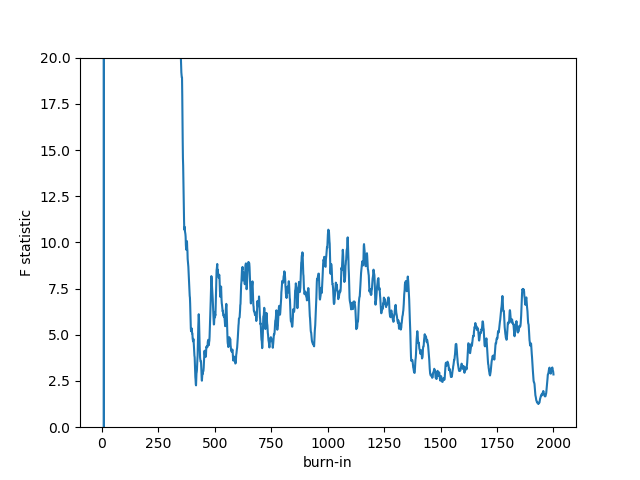
\includegraphics[width=0.45\textwidth]{f.png}
  \caption{Gelman Rubin's $F$ statistic}
  \label{fig:grs}
\end{figure}

\begin{figure}[ht]
  \centering
  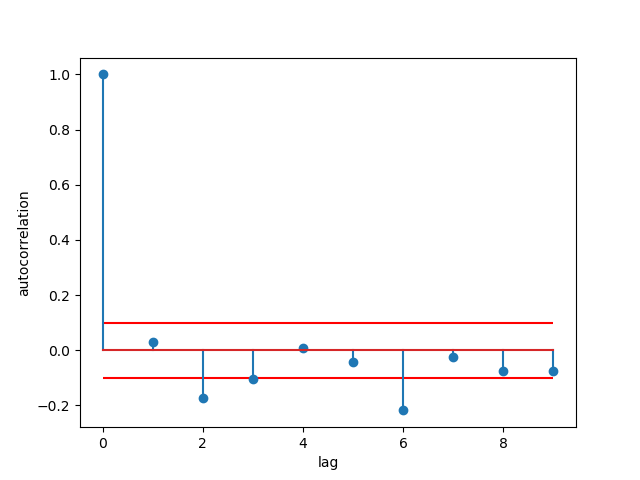
\includegraphics[width=0.45\textwidth]{batch_acf.png}
  \caption{Autocorrelation of the batches $b_1,b_2,...,b_Q$; red line = $\|{1/\sqrt{n}}\|$}
  \label{fig:batch_acf}
\end{figure}

\begin{figure*}[htp]
\centering
\begin{subfigure}[t]{0.49\textwidth}
  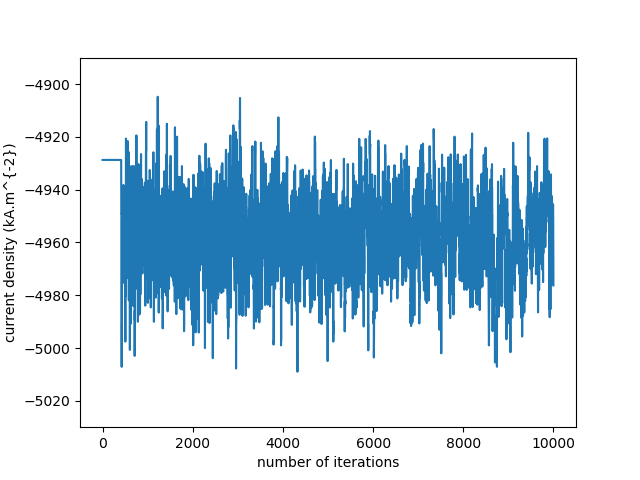
\includegraphics[width=\textwidth]{chain_2.png}
  \caption{Chain 2}
\end{subfigure}
\begin{subfigure}[t]{0.49\textwidth}
  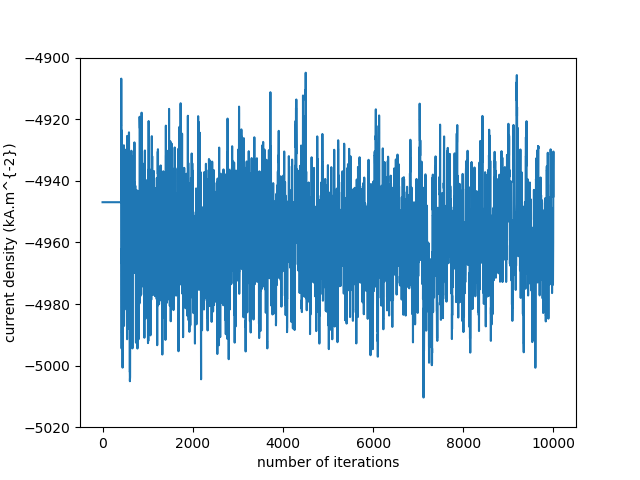
\includegraphics[width=\textwidth]{chain_3.png}
  \caption{Chain 3}
\end{subfigure}
\begin{subfigure}[t]{0.49\textwidth}
  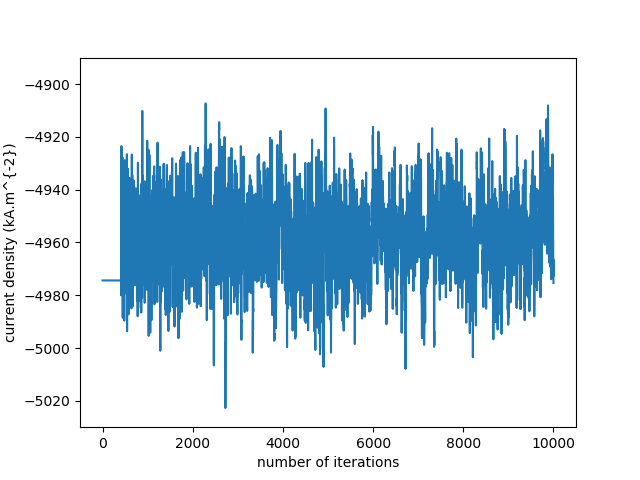
\includegraphics[width=\textwidth]{chain_4.png}
  \caption{Chain 4}
\end{subfigure}
\begin{subfigure}[t]{0.49\textwidth}
  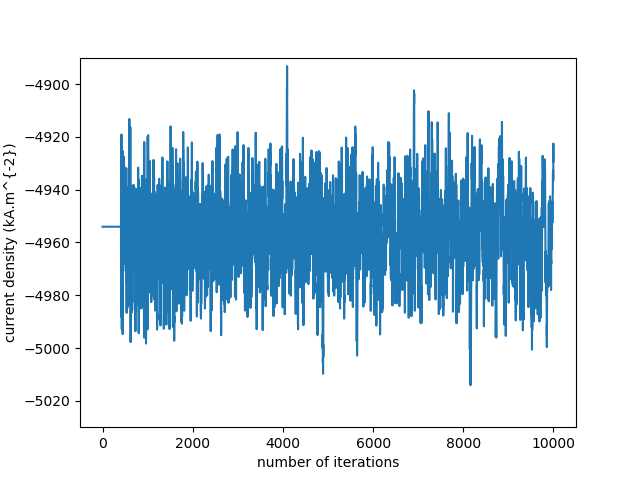
\includegraphics[width=\textwidth]{chain_5.png}
  \caption{Chain 5}
\end{subfigure}
\caption{Various chains with different initial points}
\label{fig:chains}
\end{figure*}

The error in the sample mean of the chain is called the Monte Carlo error, similar to the standard error. However independence between samples cannot be assumed here so batching is one way to cater for this \citep{geyer2011mcmc}. In batching, the chain is spilt into $Q$ non-overlapping batches of sizes $l_1,l_2,\dotdotdot,l_Q$. Let $b_1,b_2,\dotdotdot,b_Q$ be the sample mean for each of the batches, then the Monte Carlo error is
\begin{equation}
\widehat{\sigma}_{\text{ME}}=
\sqrt{
  \dfrac{
    \sum_{i=1}^Ql_i(b_i-\bar{x})^2
  }
  {
    Qn
  }
}
\ .
\end{equation}

The number of batches should increase with $n$.A good rule of thumb is to set $Q=\text{round}(\sqrt{n})$ and the batch sizes to be as similar as possible \citep{jones2006fixed}. The batch means $b_1,b_2,\dotdotdot,b_Q$ should be as uncorrelated as possible and an autocorrelation plot can be used to judge this, as shown in Figure \ref{fig:batch_acf}. 

The Monte Carlo error can be used to judge how long a chain should run. The longer the chain, the smaller the Monte Carlo error is. It can be argued that not much can be gained if the Monte Carlo error is smaller than the sample standard deviation of the chain $s$ by an order of magnitude of 2. Following from this, a threshold can be used to stop the chain, for example if $\widehat{\sigma}_{\text{ME}}/s<10^{-2}$ or $\ln(s)-\ln(\widehat{\sigma}_{\text{ME}}) > 4.6$.

The posterior mean and error, efficiency and the log Monte Carlo error are shown in Table \ref{table:diagnostic}. All 5 chains agree the estimate of the current density is $(-4.96 \pm 0.02) \text{ MA.m}^{-2}$.

\begin{table*}[htp]
\centering
\begin{tabular}{c|c|c|c}
Chain Number & Current Density $\text{ MA.m}^{-2}$ & Efficiency & $\ln(s)-\ln(\widehat{\sigma}_{\text{ME}})$ \\
\hline
1 & $-4.96 \pm 0.02$ & 0.07 & 3.4\\
2 & $-4.96 \pm 0.02$ & 0.01 & 3.2\\
3 & $-4.96 \pm 0.01$ & 0.07 & 3.4\\
4 & $-4.96 \pm 0.02$ & 0.04 & 3.2\\
5 & $-4.96 \pm 0.02$ & 0.07 & 3.3\\
\end{tabular}
\caption{Various diagnostics of the chains. The current density and the Monte Carlo error calculations discarded the first 410 samples.}
\label{table:diagnostic}
\end{table*}

\section{Java Implementation}

\begin{figure}[ht]
  \centering
  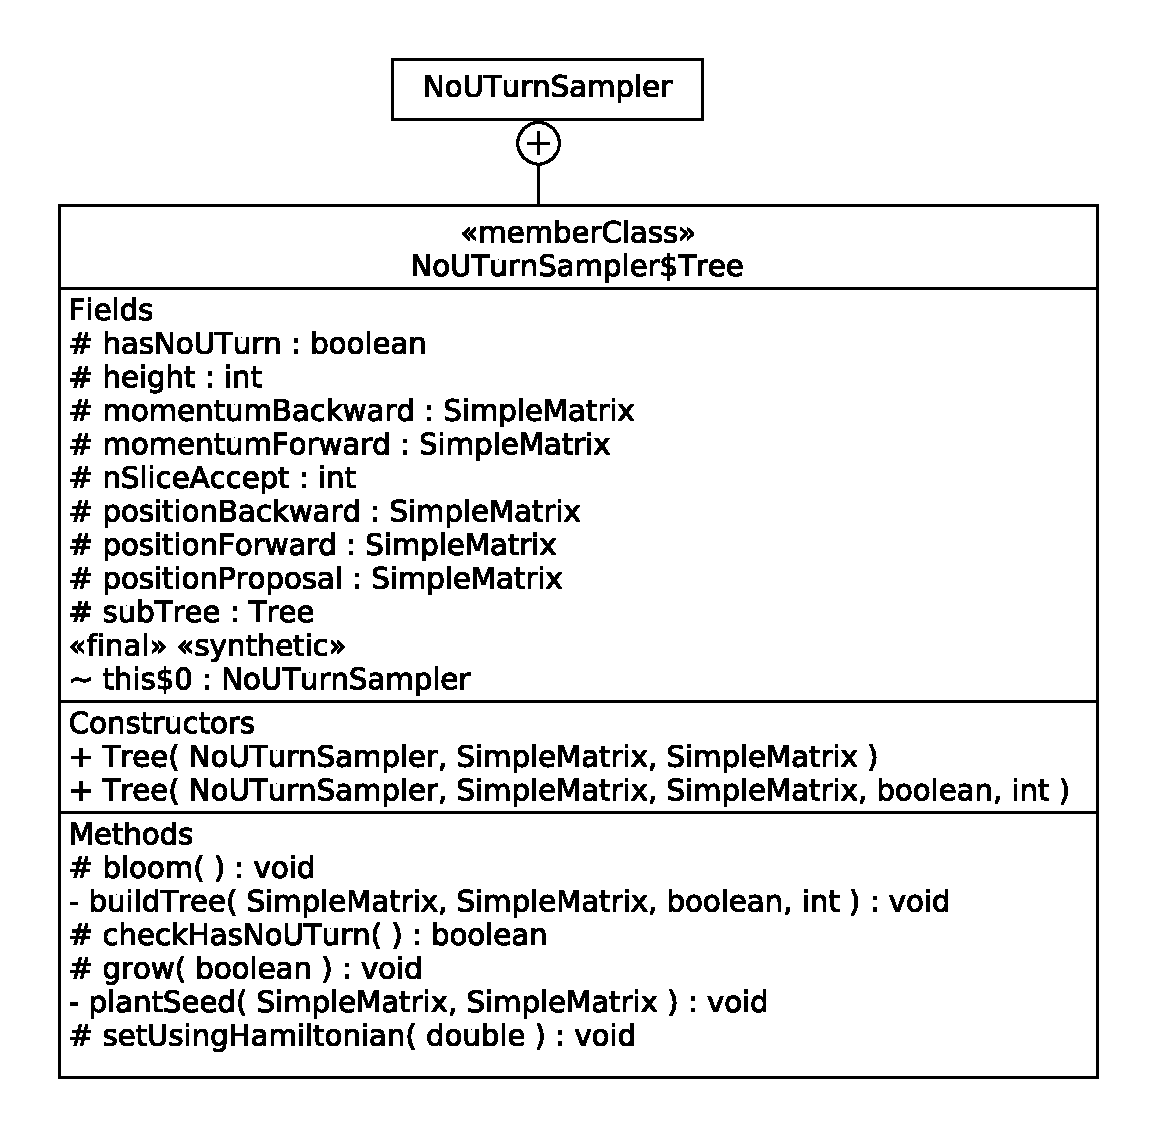
\includegraphics[width=0.45\textwidth]{NoUTurnSampler.eps}
  \caption{UML diagram of the inner class \texttt{Tree}}
  \label{fig:tree_uml}
\end{figure}

\begin{figure*}[htp]
\centering
\begin{subfigure}[t]{0.49\textwidth}
  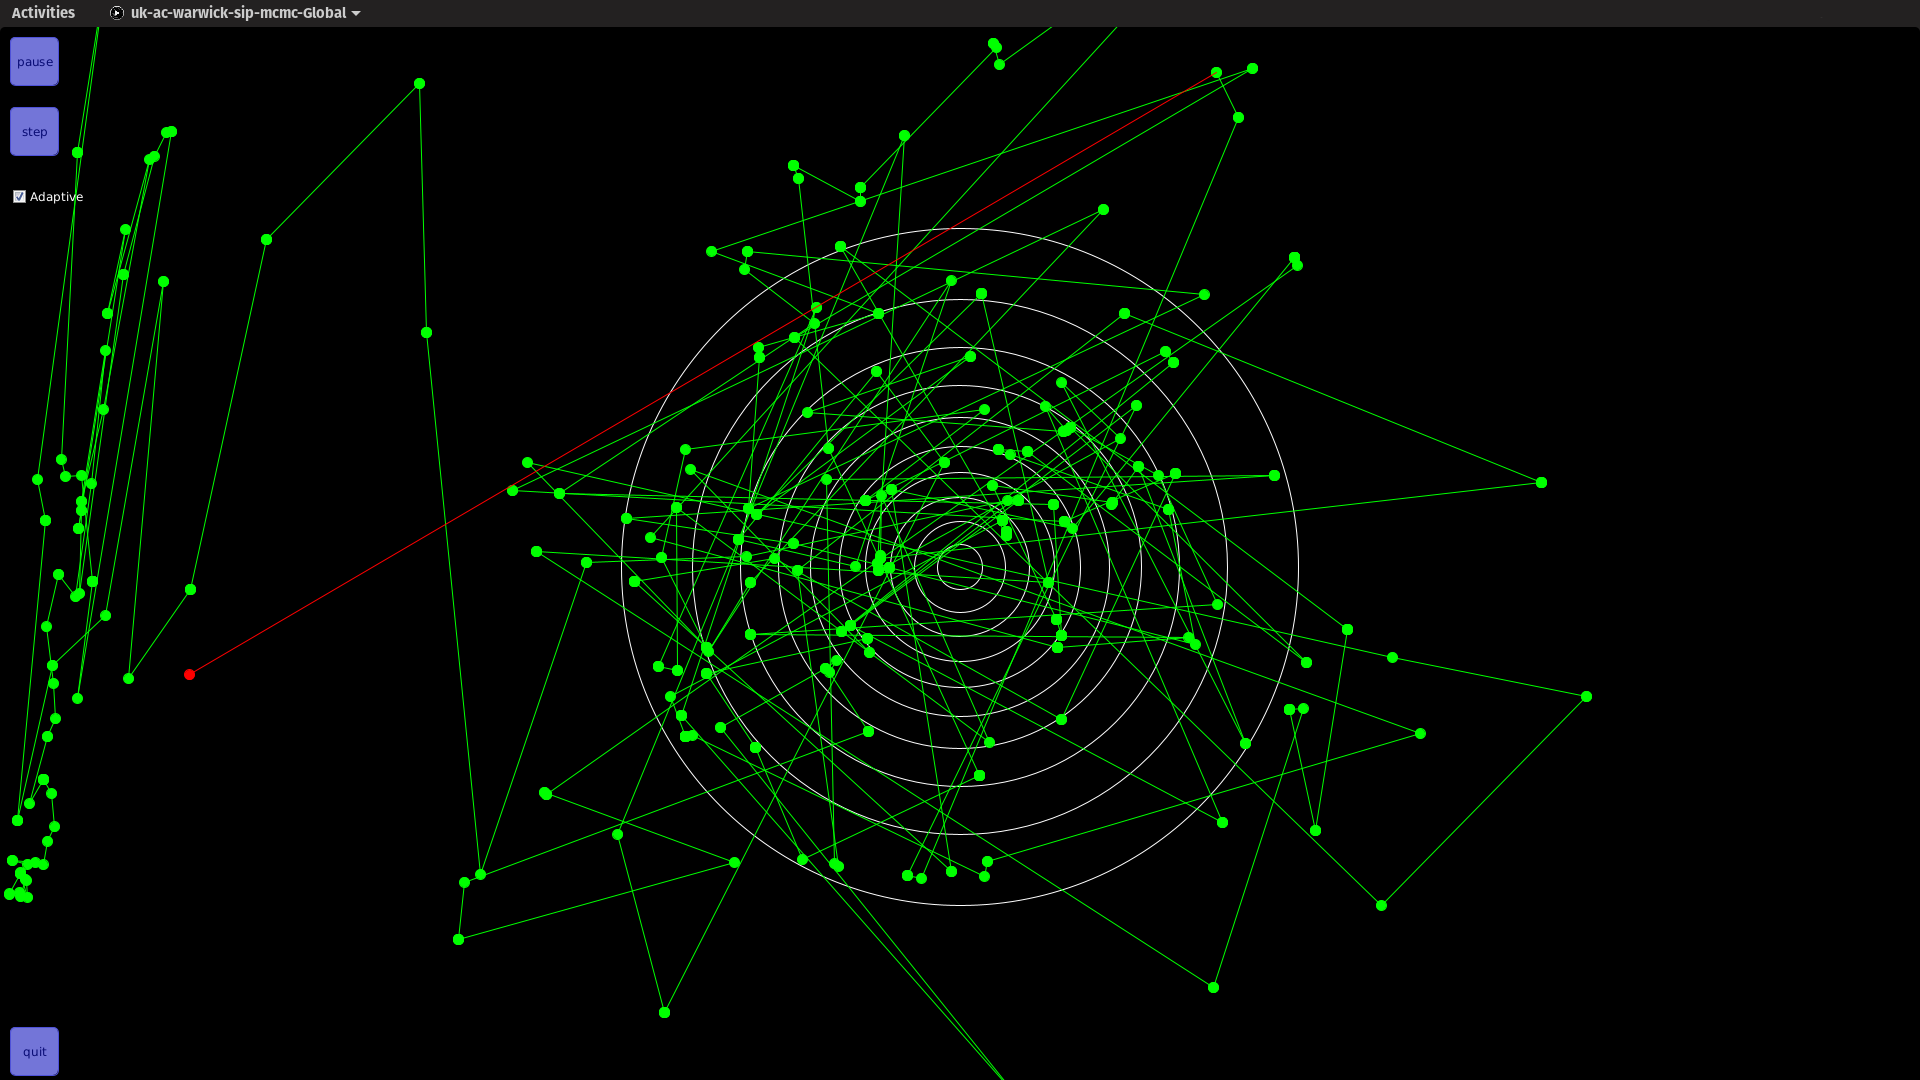
\includegraphics[width=\textwidth]{processing_rwmh.png}
  \caption{Adaptive RWMH}
\end{subfigure}
\begin{subfigure}[t]{0.49\textwidth}
  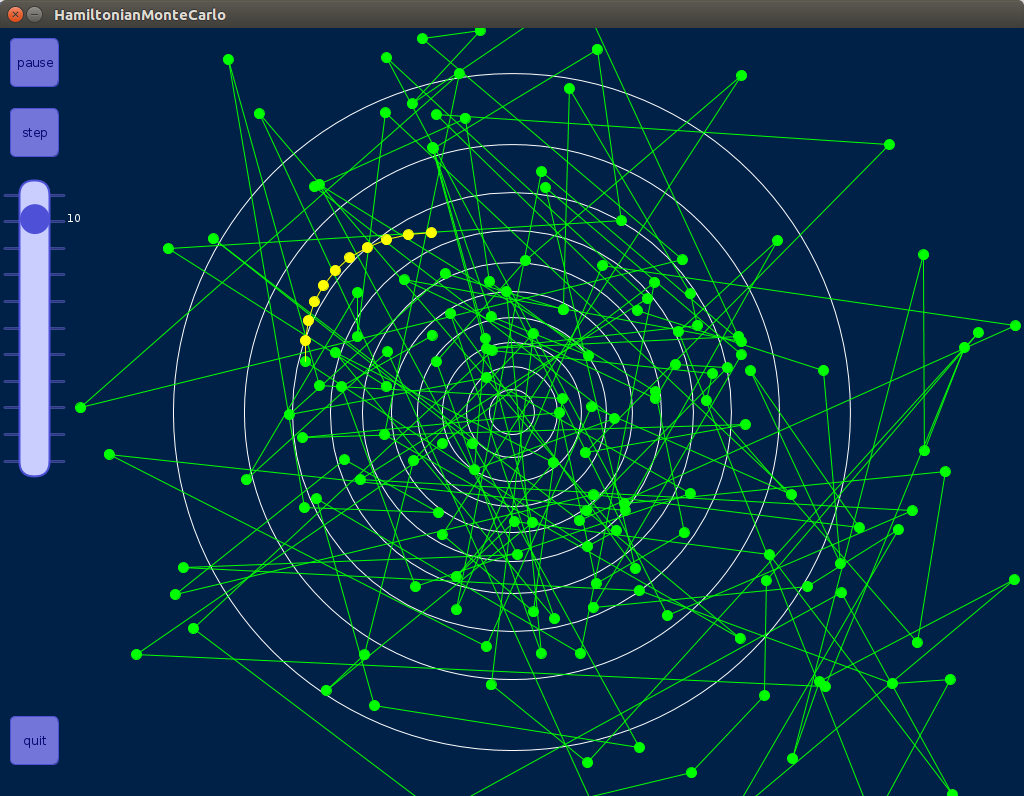
\includegraphics[width=\textwidth]{processing_hmc.png}
  \caption{HMC with sensible $L$}
\end{subfigure}
\begin{subfigure}[t]{0.49\textwidth}
  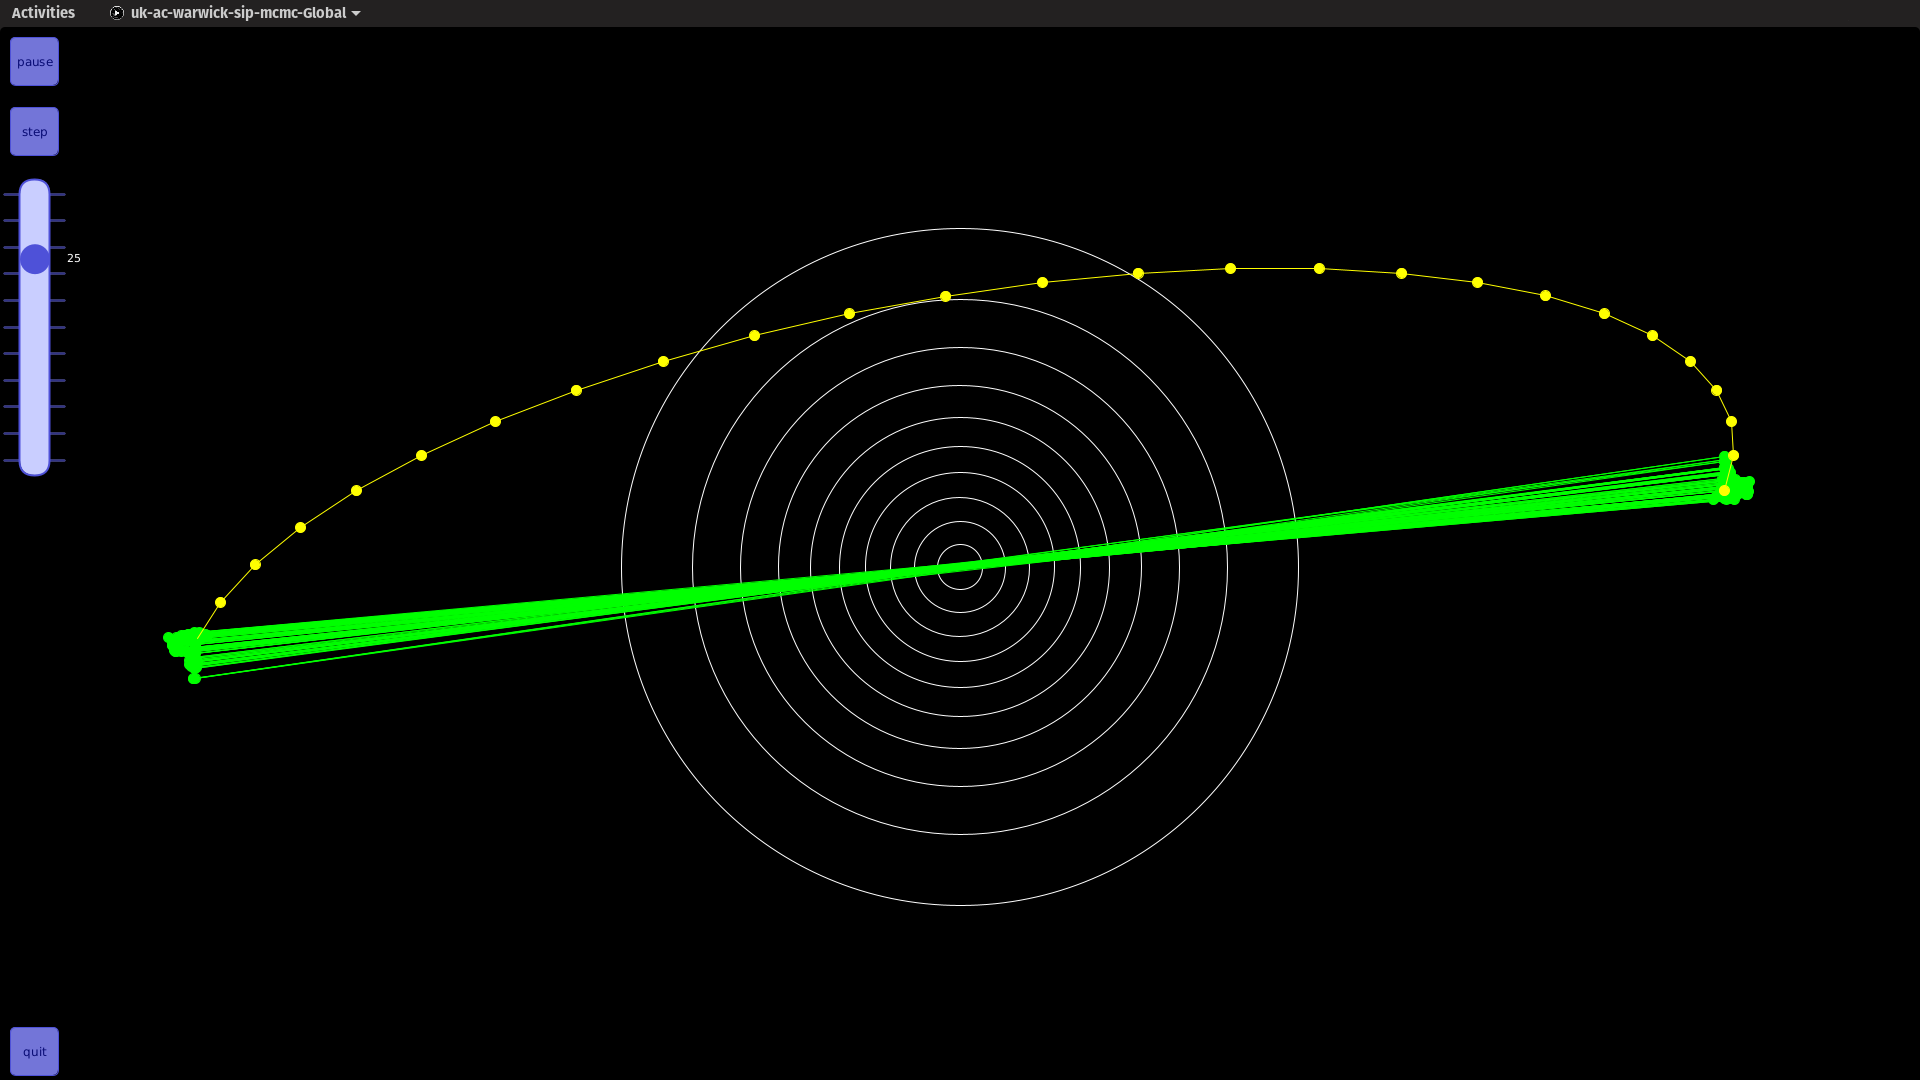
\includegraphics[width=\textwidth]{processing_hmc2.png}
  \caption{HMC with insensible $L$}
\end{subfigure}
\begin{subfigure}[t]{0.49\textwidth}
  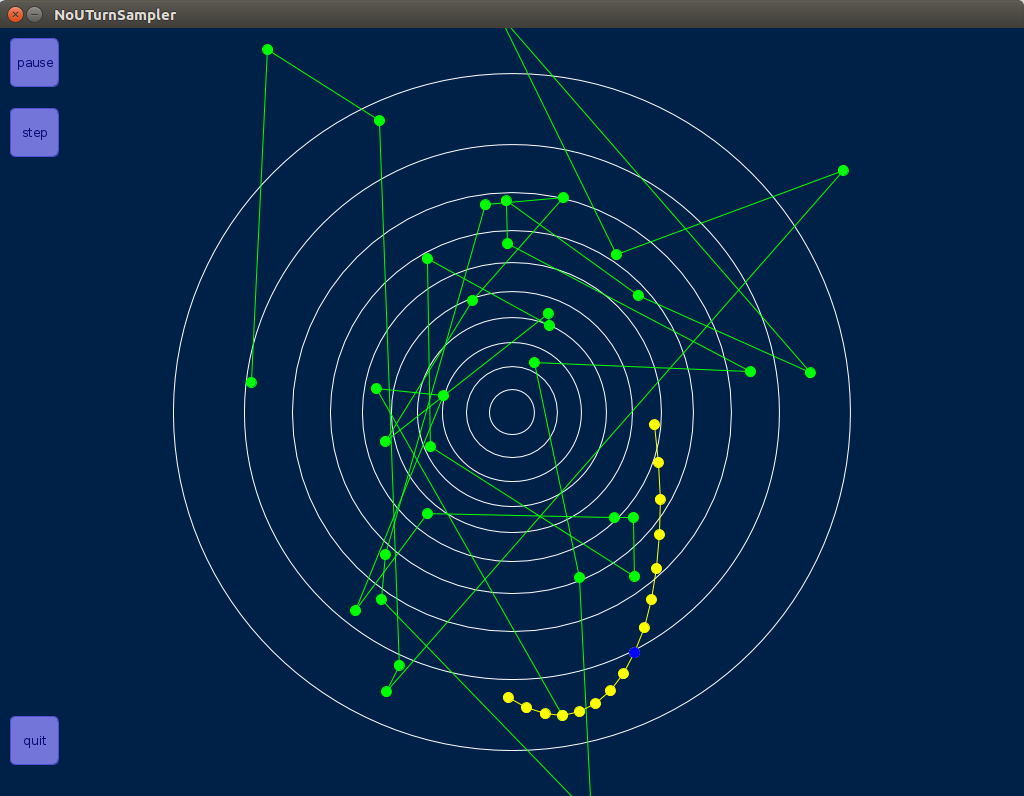
\includegraphics[width=\textwidth]{processing_nuts.png}
  \caption{NUTS}
\end{subfigure}
\caption{Various screen-shots of the visual simulation of MCMC targeting a 2D Gaussian. a) A rejected step is shown in red. b) c) Leap frog steps are shown in yellow. d) The proposal position is shown in blue.}
\label{fig:processing}
\end{figure*}

RWMH, adaptive RWMH, HMC and NUTS all have been implemented in Java. Libraries were used such as Efficient Java Matrix Library \citep{abeles2018ejml} for matrices and Apache Commons Mathematics \citep{apache2016math} for the Mersenne Twister random number generator \citep{matsumoto1998mersenne} and the one-way ANOVA. Implementation is straight forward except for NUTS because \cite{hoffman2014no} presented the algorithm using functions which returns multiple values.

Within the spirit of Java, object oriented programming was used to implement the binary tree used in NUTS. In particular the class \texttt{Tree} is an inner class of \texttt{NoUTurnSampler}. This means that an instant of \texttt{Tree} can only be instantiated by an instance of \texttt{NoUTurnSampler}. An instantiated \texttt{Tree} can access all member variables of the \texttt{NoUTurnSampler} instance which instantiated it. The \texttt{Tree} class is presented in Figure \ref{fig:tree_uml}. A short description of the class \texttt{Tree} is given here, the full source code of both classes can be found in the repository.

The objective of the \texttt{Tree} class is to grow a binary tree recursively, keep track of variables such as the forward/backward position/momentum $\vect{x}_n^-,\vect{p}_n^+,\vect{x}_n^+,\vect{p}_n^+$ and the proposal $\vect{x}_{n+1}$. It also keep tracks if the particle has satisfy the U-Turn condition.

The class has two constructors. The first one requires two parameters: the position $\vect{x}$ and momentum $\vect{p}$. It simply calls the method \texttt{plantSeed} which instantiate and initialise $\vect{x}_n^-, \vect{x}_n^+, \vect{x}_{n+1} \leftarrow \vect{x}$ and $\vect{p}_n^-, \vect{p}_n^+ \leftarrow \vect{p}$. The second constructor requires in addition a boolean to indicate the direction of growth and an integer which indicate the height of the tree. It calls the method \texttt{buildTree} which is similar to the function with the same name in \cite{hoffman2014no}. It recursively updates the forward/backward position/momentum member variables using leap frog steps and updates the proposal position accordingly.

Next the \texttt{grow} and \texttt{bloom} methods are described, both required by the \texttt{buildTree} method. The \texttt{grow} method requires a boolean parameter which indicates the direction of the growth. The method instantiate a \texttt{Tree} which grows from $\vect{x}_n^{+/-}, \vect{p}_n^{+/-}$, depending on the direction of the growth, of height \texttt{height}. This instantiated \texttt{Tree} is saved as a member variable \texttt{subTree} and is used to update the member variables  $\vect{x}_n^{+/-}, \vect{p}_n^{+/-}$ and $\vect{x}_{n+1}$. The \texttt{bloom} method is used to update the member variables \texttt{height} and \texttt{hasNoUTurn} and should be called after every \texttt{grow} call. They are in separate methods so that calculations can be done between the calls.

In the NUTS implementation, an instance of \texttt{NoUTurnSampler} instantiate a \texttt{Tree}. A while loop is used to check if \texttt{tree.hasNoUTurn}. At each iteration, a random boolean is generated to set the direction of growth. The method \texttt{tree.grow(boolean)} is called and set \texttt{tree.positionProposal = tree.subTree.positionProposal}. This is followed by a \texttt{tree.bloom()} call ready for the next iteration.

The Processing library \citep{reas2007processing} was used to create a visual simulation of the different types of MCMC targeting a 2D Gaussian. Screen-shots are shown in Figure \ref{fig:processing}.

\section{Discussion}
HMC and NUTS do struggle here because the potential energy of the posterior is not available in closed form yet. In particular it is difficult to get the numerical differentiation right for all dimensions for HMC to even work. Numerical differentiation can also be slow as it requires the evaluation of the target density for every dimension for every leap frog step, these evaluations could be put to better use in adaptive RWMH.

It should be noted that when comparing HMC with RWMH, the number of times the density or potential are evaluated should be considered, for example HMC evaluates the potential $L$ times for each sample. A fair comparison would be to comparing HMC with RWMH with thinning of $L$, that is discarding $L$ samples for every sample. In practice, thinning is not recommended \citep{geyer1992practical}.

The tuning of the mass matrix $\matr{M}$ and the step size $\Delta t$ was omitted here but discussed by \cite{hoffman2014no}. A good $\matr{M}$ would be equal to the covariance of the target so that proposal momenta are similar to the target in scale. A preliminary run using RWMH could be used to get a good value of $\matr{M}$. The tuning of $\Delta t$ was proposed using dual averaging by \cite{hoffman2014no}.

There exist extensions to HMC such as the Riemann manifold HMC \citep{girolami2011riemann} and relativistic HMC \citep{lu2016relativistic}. Outside of Java, software such as Stan \citep{carpenter2017stan} implemented and uses HMC and NUTS for the purpose of full Bayesian statistical inference and market itself as a probabilistic programming language. It can be interacted through MATLAB, C++, Python, R and other languages but Java.

The number of dimensions in current tomography under the assumption of equilibrium can get very large quickly, especially for grids finer than $3\times 3$. At that stage, long MCMC runs are required overnight. Other MCMC methods should be investigated such as for example the zig-zag process \citep{bierkens2016zig}, bouncy particle filter \citep{bouchard2018bouncy} and the scalable Langevin exact algorithm \citep{pollock2016scalable}.

\section{Code Repository}
The code is available in the repository under the Apache License 2.0 \url{https://github.com/shermanip/oxwasp_exchange_mcmc}. There exist two branches, one for visualising MCMC \url{https://github.com/shermanip/oxwasp_exchange_mcmc/tree/processing}, the other implements MCMC on the equilibrium problem but requires software and data only available to staff at Culham Centre for Fusion Energy \url{https://github.com/shermanip/oxwasp_exchange_mcmc/tree/ccfe}.

\bibliographystyle{apalike}
\bibliography{bib}

\end{document}
